\section{The Radix-$2^3$ FFT  Algorithm}
\begin{frame}
  \frametitle{\textbf{Table of Contents}}
  \begin{center}
    {\vspace{-1.5cm}\Large \textbf{Section \thesection}\vspace{0.5cm}}
    \begin{beamercolorbox}[
      sep=8pt,center]{part title}
      \usebeamerfont{part title}
      \textbf{\insertsection}
    \end{beamercolorbox}
  \end{center}
\end{frame}

\begin{frame}
	\frametitle{\textbf{The Radix-$2^3$ FFT  Algorithm}}
	\framesubtitle{\secname : \subsecname}
	\begin{block}{\centering \textbf{\textit{N}-point DFT of an input sequence $x[n]$}}
		\begin{equation}
			X[k] = \sum_{n=0}^{N-1} x[n] \cdot W_N^{nk}, \quad k=0,1,...,N-1 \qquad
		\end{equation}
		where $W_N^{nk} = e^{-j\frac{2\pi}{N} nk}$. 
	\end{block}
	
	\begin{block}{\centering}
		\begin{itemize}\justifying\footnotesize
			\item Direct computation of the DFT is inefficient because it does not exploit the properties of:
			\begin{enumerate}
				\item Symmetry: $ W_N^{k+N/2} = -W_N^k$
				\item Periodicity:  $W_N^{k+N} = W_N^k$
			\end{enumerate}
			\item The FFT based on Cooley-Tukey algorithm reduce the number of operations from $O(N^2)$ for the DFT to $O(Nlog_2N)$ for the FFT.
		\end{itemize}	
	\end{block}
\end{frame}


\begin{frame}
  	\frametitle{\textbf{The Radix-$2^3$ FFT  Algorithm}}
	\framesubtitle{\secname : \subsecname}
	\begin{block}{\centering \textbf{\textit{Divide and Conquer} approach}}
		\begin{itemize} \justifying\footnotesize		
			\item We can calculate the DFT in series of $s=log_\rho N$ stages, where $\rho$ is the base of the \textit{radix}. 
			\item This is based on the decomposition of an N point DFT into successively smaller DFTs.
			\item  In our case, the numeber of stages is:
		 	\begin{equation}
		 			s = log_2 (128) = 7 
		 	\end{equation}
		\end{itemize}		
	\end{block}

	\begin{block}{\centering \textbf{Methods to design FFT algorithms}}
		\begin{enumerate} \justifying\footnotesize
			\item \textbf{Decimation In Time (DIT):} Splitting successively data sequence $x[n]$ by a factor of 2. 					
			\item \textbf{Decimation In Frcuency (DIF):} Splitting successively the data sequence $X[k]$ by a factor of 2. 
		\end{enumerate}											
  	\end{block}
\end{frame}

\begin{frame}
  	\frametitle{\textbf{The Radix-$2^3$ FFT  Algorithm}}
	\framesubtitle{\secname : \subsecname}
	\begin{block}{\centering \textbf{DIT and DIF Butterflies}}
		The difference is the instant in which the multiplication by $W_N^\phi$ is accomplished. 
	\end{block}    	
    	\vspace{-0.2cm}
    	\begin{figure}[h!] \centering
    		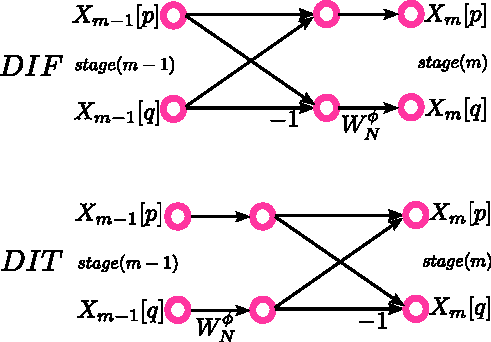
\includegraphics[width=0.45\paperwidth]{./image/DifDit.pdf}
    	\end{figure}
\end{frame}

\begin{frame}
  	\frametitle{\textbf{The Radix-$2^3$ FFT  Algorithm}}
	\framesubtitle{\secname : \subsecname}
	\begin{block}{\centering \textbf{Order of samples in DIT and DIF}}
		\begin{itemize}\justifying\footnotesize
			\item  The input samples in FFT algorithms DIF are organized in natural order but its output has not in order.
			\item The opposite is for DIT.
		\end{itemize}
	\end{block}    	
    \begin{figure}[h!] \centering
    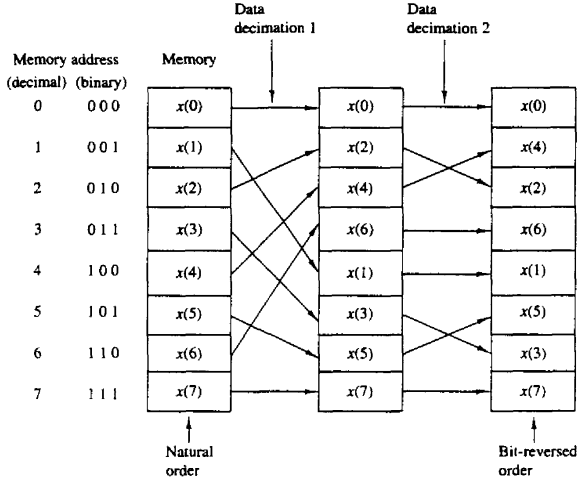
\includegraphics[width=0.4\paperwidth]{./image/dif_order.png}
    	\caption{\footnotesize Order of intpus and outputs for DIF FFT.} % Añadir referencia
    \end{figure}
\end{frame}



\begin{frame}
  	\frametitle{\textbf{The Radix-$2^3$ FFT  Algorithm}}
	\framesubtitle{\secname : \subsecname}
	\begin{block}{\centering \textbf{Mathematic expression of radix-8 butterfly element}}
		\vspace{-0.3cm}		 
		 \scalebox{0.55}{
			\label{eqn:radix}		 
		 \parbox{\linewidth}{    		
		\begin{align}			
		C_{8k+0} = \sum_{n=0}^{N/8-1} \bigg\{&[(x_n + x_{n+\frac{N}{2}}) + (x_{n+\frac{N}{4}} + x_{n+\frac{3N}{4}})] + [(x_{n+\frac{N}{8}} + x_{n+\frac{5N}{8}}) + (x_{n+\frac{3N}{8}} + x_{n+\frac{7N}{8}})] \bigg\} W_N^{0n} W_{N/8}^ {nk}     \nonumber \\
		%	
		C_{8k+4} = \sum_{n=0}^{N/8-1} \bigg\{&[(x_n + x_{n+\frac{N}{2}}) + (x_{n+\frac{N}{4}} + x_{n+\frac{3N}{4}})] - [(x_{n+\frac{N}{8}} + x_{n+\frac{5N}{8}}) + (x_{n+\frac{3N}{8}} + x_{n+\frac{7N}{8}})] \bigg\} W_N^{4n} W_{N/8}^ {nk}     \nonumber\\
		%
		C_{8k+2} = \sum_{n=0}^{N/8-1} \bigg\{&[(x_n + x_{n+\frac{N}{2}}) - (x_{n+\frac{N}{4}} + x_{n+\frac{3N}{4}})] -j [(x_{n+\frac{N}{8}} + x_{n+\frac{5N}{8}}) - (x_{n+\frac{3N}{8}} + x_{n+\frac{7N}{8}})] \bigg\} W_N^{2n} W_{N/8}^ {nk}     \nonumber\\
		%
		C_{8k+6} = \sum_{n=0}^{N/8-1} \bigg\{&[(x_n + x_{n+\frac{N}{2}}) - (x_{n+\frac{N}{4}} + x_{n+\frac{3N}{4}})] +j	[(x_{n+\frac{N}{8}} + x_{n+\frac{5N}{8}}) - (x_{n+\frac{3N}{8}} + x_{n+\frac{7N}{8}})] \bigg\} W_N^{6n} W_{N/8}^ {nk}     \nonumber\\
		%
		C_{8k+1} = \sum_{n=0}^{N/8-1} \bigg\{&[(x_n - x_{n+\frac{N}{2}}) -j (x_{n+\frac{N}{4}} - x_{n+\frac{3N}{4}})] + W_N^{N/8} [(x_{n+\frac{N}{8}} - x_{n+\frac{5N}{8}}) -j (x_{n+\frac{3N}{8}} - x_{n+\frac{7N}{8}})] \bigg\} W_N^{n} W_{N/8}^ {nk}     \nonumber\\
		%
		C_{8k+5} = \sum_{n=0}^{N/8-1} \bigg\{&[(x_n - x_{n+\frac{N}{2}}) -j (x_{n+\frac{N}{4}} - x_{n+\frac{3N}{4}})] - W_N^{N/8} [(x_{n+\frac{N}{8}} - x_{n+\frac{5N}{8}}) -j (x_{n+\frac{3N}{8}} - x_{n+\frac{7N}{8}})] \bigg\} W_N^{5n} W_{N/8}^ {nk}    \nonumber\\
		%
		C_{8k+3} = \sum_{n=0}^{N/8-1} \bigg\{&[(x_n - x_{n+\frac{N}{2}}) +j (x_{n+\frac{N}{4}} - x_{n+\frac{3N}{4}})] + W_N^{3N/8} [(x_{n+\frac{N}{8}} - x_{n+\frac{5N}{8}}) +j (x_{n+\frac{3N}{8}} - x_{n+\frac{7N}{8}})] \bigg\} W_N^{3n} W_{N/8}^ {nk}    \nonumber\\
		%
		C_{8k+7} = \sum_{n=0}^{N/8-1} \bigg\{&[(x_n - x_{n+\frac{N}{2}}) +j (x_{n+\frac{N}{4}} + x_{n+\frac{3N}{4}})] - W_N^{3N/8} [(x_{n+\frac{N}{8}} - x_{n+\frac{5N}{8}}) +j (x_{n+\frac{3N}{8}} - x_{n+\frac{7N}{8}})] \bigg\} W_N^{7n} W_{N/8}^ {nk}    \nonumber 	
		\end{align}}}
	\end{block}
    
    
\end{frame}

\begin{frame}
  	\frametitle{\textbf{The Radix-$2^3$ FFT  Algorithm}}
	\framesubtitle{\secname : \subsecname}
	\begin{block}{\centering \textbf{Radix-$2^k$ Implementation}}
		The quantity of rotators of an architecture radix-$2^k$ (with $k>1$) is less than the radix-2.
	\end{block}
    \begin{figure}[h!] \centering
    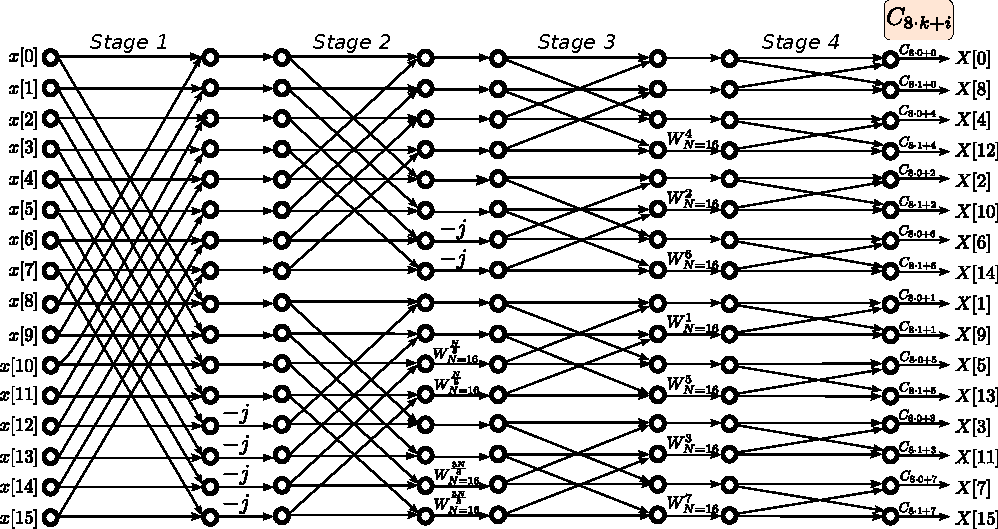
\includegraphics[width=0.75\paperwidth]{./image/16points_con.pdf}
    \caption{\footnotesize Flow graph of a radix-$2^3$ 16-point DIF DFT.}
    \end{figure}
\end{frame}
    
\begin{frame}
  	\frametitle{\textbf{The Radix-$2^3$ FFT  Algorithm}}
	\framesubtitle{\secname : \subsecname}
	

  \begin{block}{\centering \textbf{The Radix-$2^3$ FFT  Algorithm}}
    \vspace{-0.5cm}
    \begin{tabular}[c]{lr}
      %\hspace{-0.4cm}
      \begin{minipage}[t]{0.45\linewidth}
        \vspace{0.5cm}
        \begin{itemize} \justifying\footnotesize
        \item Applying (\ref{eqn:radix}) for the 128 point DFT and calculating each coefficient for $k=0,1,...,(128/8)-1$:
			\scalebox{1}{\parbox{0.45\linewidth}{    				
			\begin{equation*} 
				C_{8k+i} = \sum_{n=0}^{128/8-1} \{ \cdot \}
			\end{equation*}}}\\			         
         	We get a sequence in chain of butterflies with its corresponding rotation factor.
        \item The 128 point DFT goes through a processes that involve tree stages of butterflies to arrive finally to a set of eight DFT where each of one is a 16 point DFT.
        \end{itemize}
      \end{minipage}
      \hspace{0.3cm}
      \begin{minipage}[t]{0.45\linewidth}
        \vspace{0.5cm}
    \begin{figure}[h!] \centering
    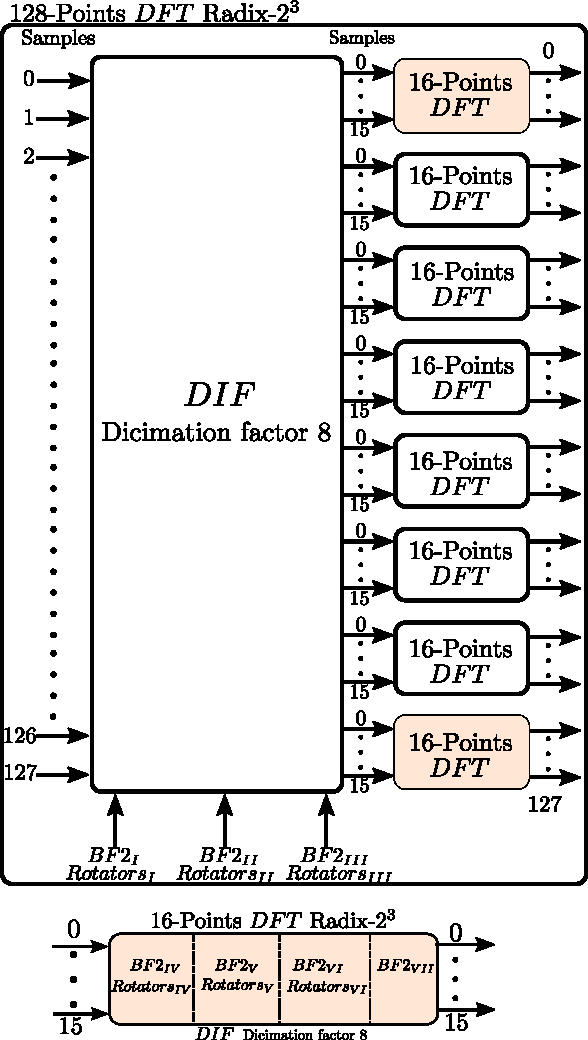
\includegraphics[height=0.6\paperheight]{./image/BloquesDft.pdf}
    \end{figure}
      \end{minipage}
    \end{tabular}
  \end{block}

\end{frame}




